\chapter{System Architecture}

This chapter describes the full HTDet pipeline, from raw image input to final detection output. The system is composed of three stages: a MobileViT-S \textit{backbone} for feature extraction, a FPN-based \textit{neck} for multi-scale feature aggregation, and a RetinaNet \textit{head} for prediction. The pipeline is illustrated in Figure \ref{fig:htdet_overview}.

\begin{figure}[H]
\centering
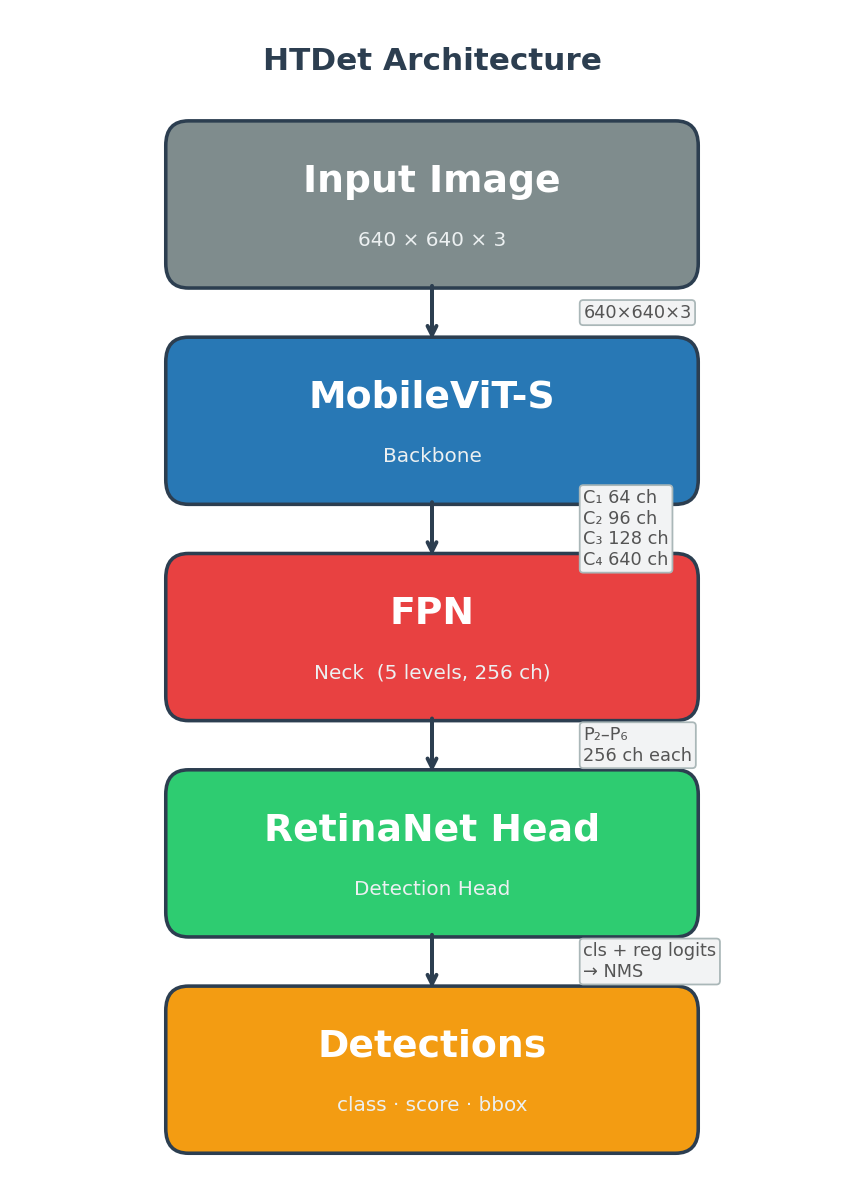
\includegraphics[width=0.55\textwidth]{images/htdet_overview.png}
\caption{HTDet system overview: MobileViT-S backbone, FPN neck, and RetinaNet head.}
\label{fig:htdet_overview}
\end{figure}

\section{Design Summary}

\begin{table}[H]
\centering
\caption{HTDet Full Model Parameter Count}
\begin{tabular}{|l|c|c|}
\hline
\textbf{Component} & \textbf{Parameters} & \textbf{GFLOPs (640$\times$640)} \\
\hline
Backbone (MobileViT-S)   & 5.58 M  & 4.65  \\
Neck (FPN, 256-ch)       & 2.9 M   & 185   \\
Head (RetinaNet, 256-ch) & 5.1 M   & 563   \\
\hline
\textbf{Total}           & \textbf{12.4 M} & \textbf{198.9} \\
\hline
\end{tabular}
\label{table:model_params}
\end{table}

\clearpage

%% ── MobileViT-S + FPN + RetinaNet (flow across pages naturally) ──────────────
\section{Backbone: MobileViT-S}

\begin{figure}[H]
\centering
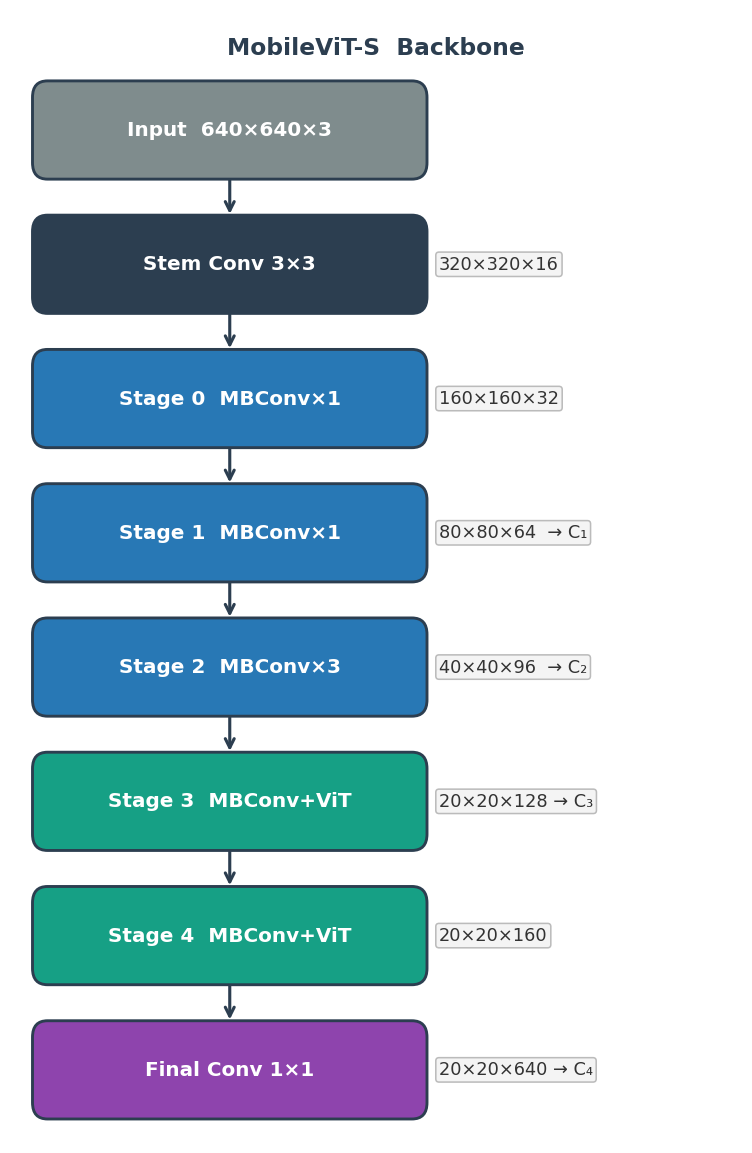
\includegraphics[width=0.52\textwidth]{images/mobilevit_backbone.png}
\caption{MobileViT-S backbone: stage-wise architecture with output feature map dimensions.}
\label{fig:backbone_diagram}
\end{figure}

The backbone is \textbf{MobileViT-S} loaded from the TIMM library with ImageNet pretrained weights:

\begin{verbatim}
type='TIMMBackbone', model_name='mobilevit_s', pretrained=True
\end{verbatim}

MobileViT-S was selected over lighter variants (MobileViT-XS, MobileViT-XXS) because the URPC task requires distinguishing visually similar underwater organisms in degraded conditions — a task that demands strong representational capacity. At 5.58M backbone parameters, MobileViT-S is still compact enough for FPGA deployment.

The backbone exports four feature maps that serve as FPN inputs:

\begin{table}[H]
\centering
\caption{MobileViT-S Feature Map Outputs (for $640\times640$ input)}
\begin{tabular}{|c|c|c|c|}
\hline
\textbf{Feature} & \textbf{Resolution} & \textbf{Channels} & \textbf{Source} \\
\hline
$C_1$ & $80\times80$  & 64  & Stage 2 \\
$C_2$ & $40\times40$  & 96  & Stage 3 \\
$C_3$ & $20\times20$  & 128 & Stage 4 \\
$C_4$ & $20\times20$  & 640 & Stage 5 (after final $1\times1$ expansion) \\
\hline
\end{tabular}
\label{table:feature_maps}
\end{table}

\section{Neck: Feature Pyramid Network}

\begin{figure}[H]
\centering
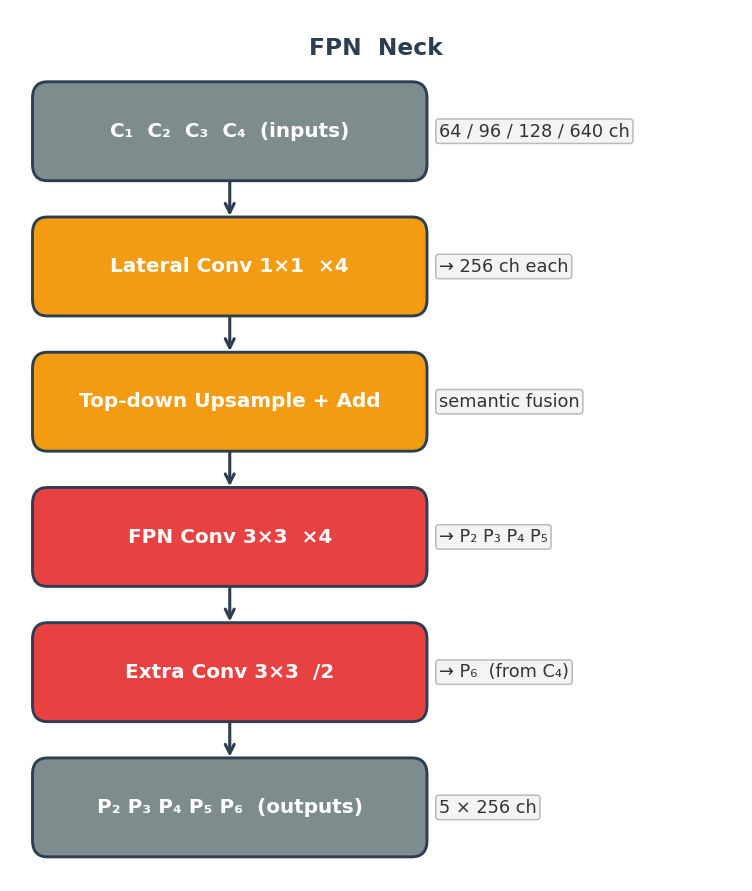
\includegraphics[width=0.52\textwidth]{images/fpn_neck.png}
\caption{FPN neck: lateral convolutions, top-down fusion, and output pyramid levels.}
\label{fig:fpn_diagram}
\end{figure}

The standard FPN takes $\{C_1, C_2, C_3, C_4\}$ and builds a 5-level pyramid $\{P_2, P_3, P_4, P_5, P_6\}$. Lateral $1\times1$ convolutions project each backbone feature to a uniform channel depth of 256. Top-down upsampling then adds high-level semantics to lower-level features, so every output level carries both fine spatial detail and global context. $P_6$ is generated directly from $C_4$ via a stride-2 $3\times3$ convolution to extend coverage to very large objects.

Each FPN output level has 256 channels and is passed independently to the shared detection head. For the compact FPGA deployment model ($192\times192$ input), the channel depth is reduced to 192 to meet the low-GFLOPs design target.

\section{Detection Head: RetinaNet}

\begin{figure}[H]
\centering
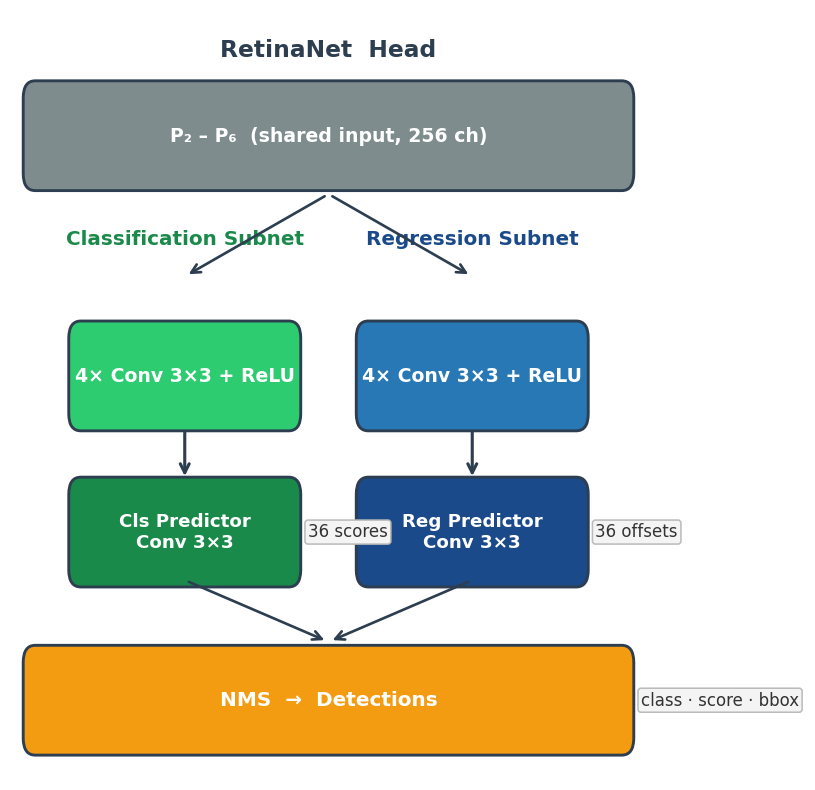
\includegraphics[width=0.55\textwidth]{images/retina_head.png}
\caption{RetinaNet detection head: parallel classification and regression subnets applied at each FPN level.}
\label{fig:head_diagram}
\end{figure}

The detection head is a standard RetinaNet head shared across all five FPN levels:

\begin{itemize}
    \item \textbf{Classification subnet:} 4 stacked $3\times3$ Conv-BN-ReLU layers, followed by a $3\times3$ classification predictor producing $K \times A$ scores (where $K=4$ classes, $A=9$ anchors per location).
    \item \textbf{Regression subnet:} 4 stacked $3\times3$ Conv-BN-ReLU layers, followed by a $3\times3$ regression predictor producing $4A$ box offsets per location.
\end{itemize}

Anchors use three scales ($2^0$, $2^{1/3}$, $2^{2/3}$) and three aspect ratios (0.5, 1.0, 2.0) at each grid point, giving 9 anchors per location. The head uses \textbf{Focal Loss} for classification and \textbf{L1 loss} for bounding box regression.
